\section{Maximum Likelihood Estimation}

In the current section,
the parameters \(\beta, \gamma, t^*\) will be considered to be distributed, according to some known distributions.
This makes the outcomes of the function \(t^{opt}(\beta, \gamma, t^*)\) defined above to be distributed themselves,
according to another probability distribution.

We explicitly characterize the distribution of the optimal arrival times,
by finding an expression for its probability density function (p.d.f.).
Once the density of the optimal arrival times \(t^{opt}\) has been found,
its evaluation can yield an expression for the likelihood of a given dataset of arrival times.
If the original distributions were parametric,
the expression allows to perform a Maximum Likelihood Estimation,
for estimating the value of the parameter the dataset was generated according to.

\subsection{Theoretical Prerequisites}


The goal of the section is thus to find an analytical expression for the Probability Density Function that characterizes the distribution of the outcomes of the function \(t^{opt}\).
To this end, the characterization developed in the preceding section will be employed,
in a slightly simpler setting, in which some additional hypotheses on the travel time function are made.

The assumptions that simplify the estimation are shown in the following definition:
\begin{definition}
  \label{def:proper_tt}
  Let \(tt_a:\R\rightarrow\R\).

  \(tt_a\) is a \textbf{Proper Travel Time Function} if \(tt_a\) is a General Travel Time Function and,
  on top of this, 
  there exist two time points \(k_1 \neq k_2 \in \R\) such that,
  in the subsets
  \begin{align}
    \label{eq:subs_conc_conv}
    \mathcal{D}_{conc} = (k_1, k_2) && \mathcal{D}_{conv} = \R \setminus \mathcal{D}_{conc}
  \end{align}
  The function \(tt_a\) satisfies the following:
  \begin{enumerate}
  \item \(tt_a\) is concave on the domain \(\mathcal{D}_{conc}\)
  \item \(tt_a\) is convex on the domain \(\mathcal{D}_{conv}\)
  \end{enumerate}
\end{definition}
\todo{Why is proper tt even realistic?}

\begin{figure}
  \centering
  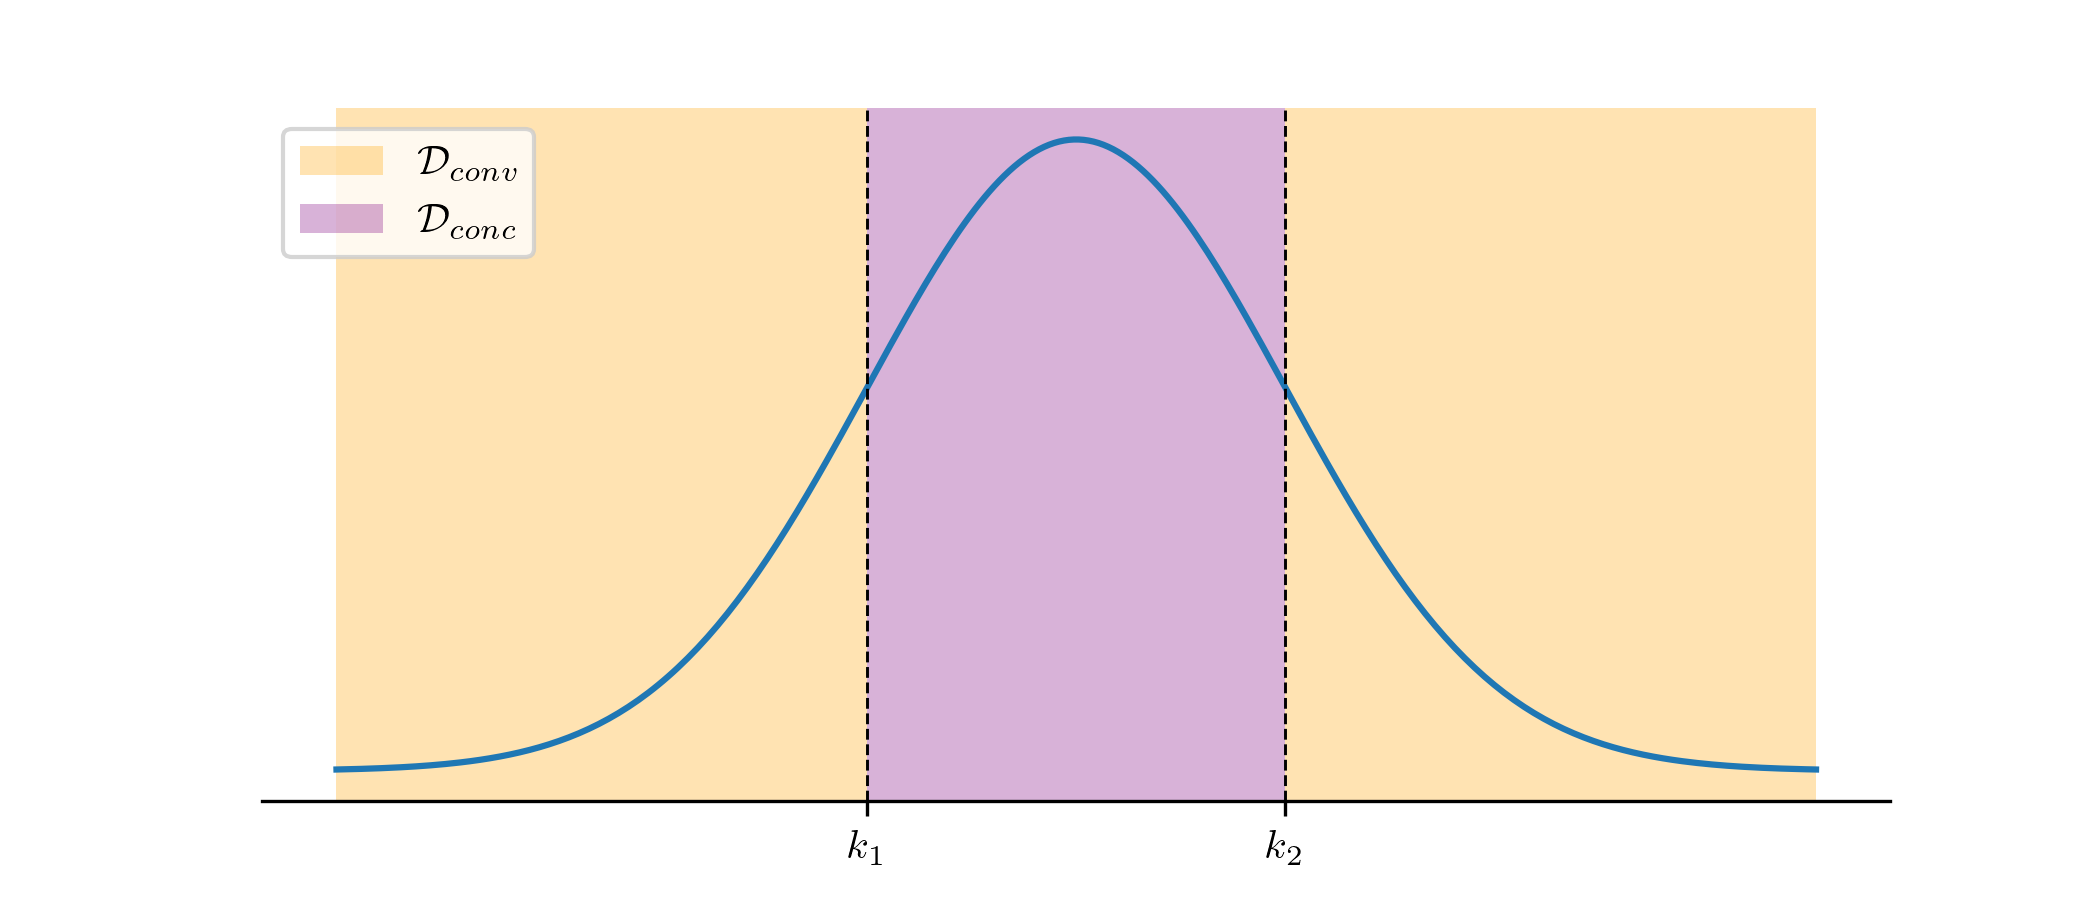
\includegraphics[width=.9\textwidth]{conv_conc_gauss}
  \caption{
    Example of a proper travel time function.
  The shaded zones show the parts of its domain in which the function is convex or concave.}
  \label{fig:conc-conv-gauss}
\end{figure}

An example of such a function is the gaussian function,
shown in Figure~\ref{fig:conc-conv-gauss} with the corresponding subsets \(\mathcal{D}_{conc}, \mathcal{D}_{conv}\).

For a proper travel time function,
the estimation of the optimal arrival time \(t^{opt}\) considerably simplifies:
the following observation shows how.
\begin{obs}
  \label{obs:simplified-char}
  Consider the problem of choosing an optimal departure time
  with a proper travel time function, and let \(\beta, \gamma\) be fixed.

  There exist two intervals \((t_i^e, t_f^e), (t_i^l, t_f^l)\) such that an on-time arrival \(t^{opt} = t^*\) is realized if and only if
  \begin{equation*}
    t^* \notin (t_i^e, t_f^e) \cup  (t_i^l, t_f^l)
  \end{equation*}
\end{obs}

Note that this is implied from what said by Proposition~\ref{prop:into-early-late},
except for a single detail:
the intervals are indeed here at most one (for each type of arrival), rather than an arbitrary number.

This is a consequence of the hypothesis on the travel time function:
the point \(t_i^e\) must indeed be an eligible early arrival and,
as shown in Lemma~\ref{lemma:bounded-der-tt} and~\ref{lemma:cost_decoupled},
any possible early arrival must satisfy two simple conditions:
\begin{enumerate}
\item \(tt_a'(t_i^e) = \beta\)
\item \(tt_a''(t_i^e) \geq 0\)
\end{enumerate}
where the second one derives from it being a minimum:
if the second derivative was negative, the point was indeed a local maximum and thus not a minimizer.

\begin{figure}
  \centering
  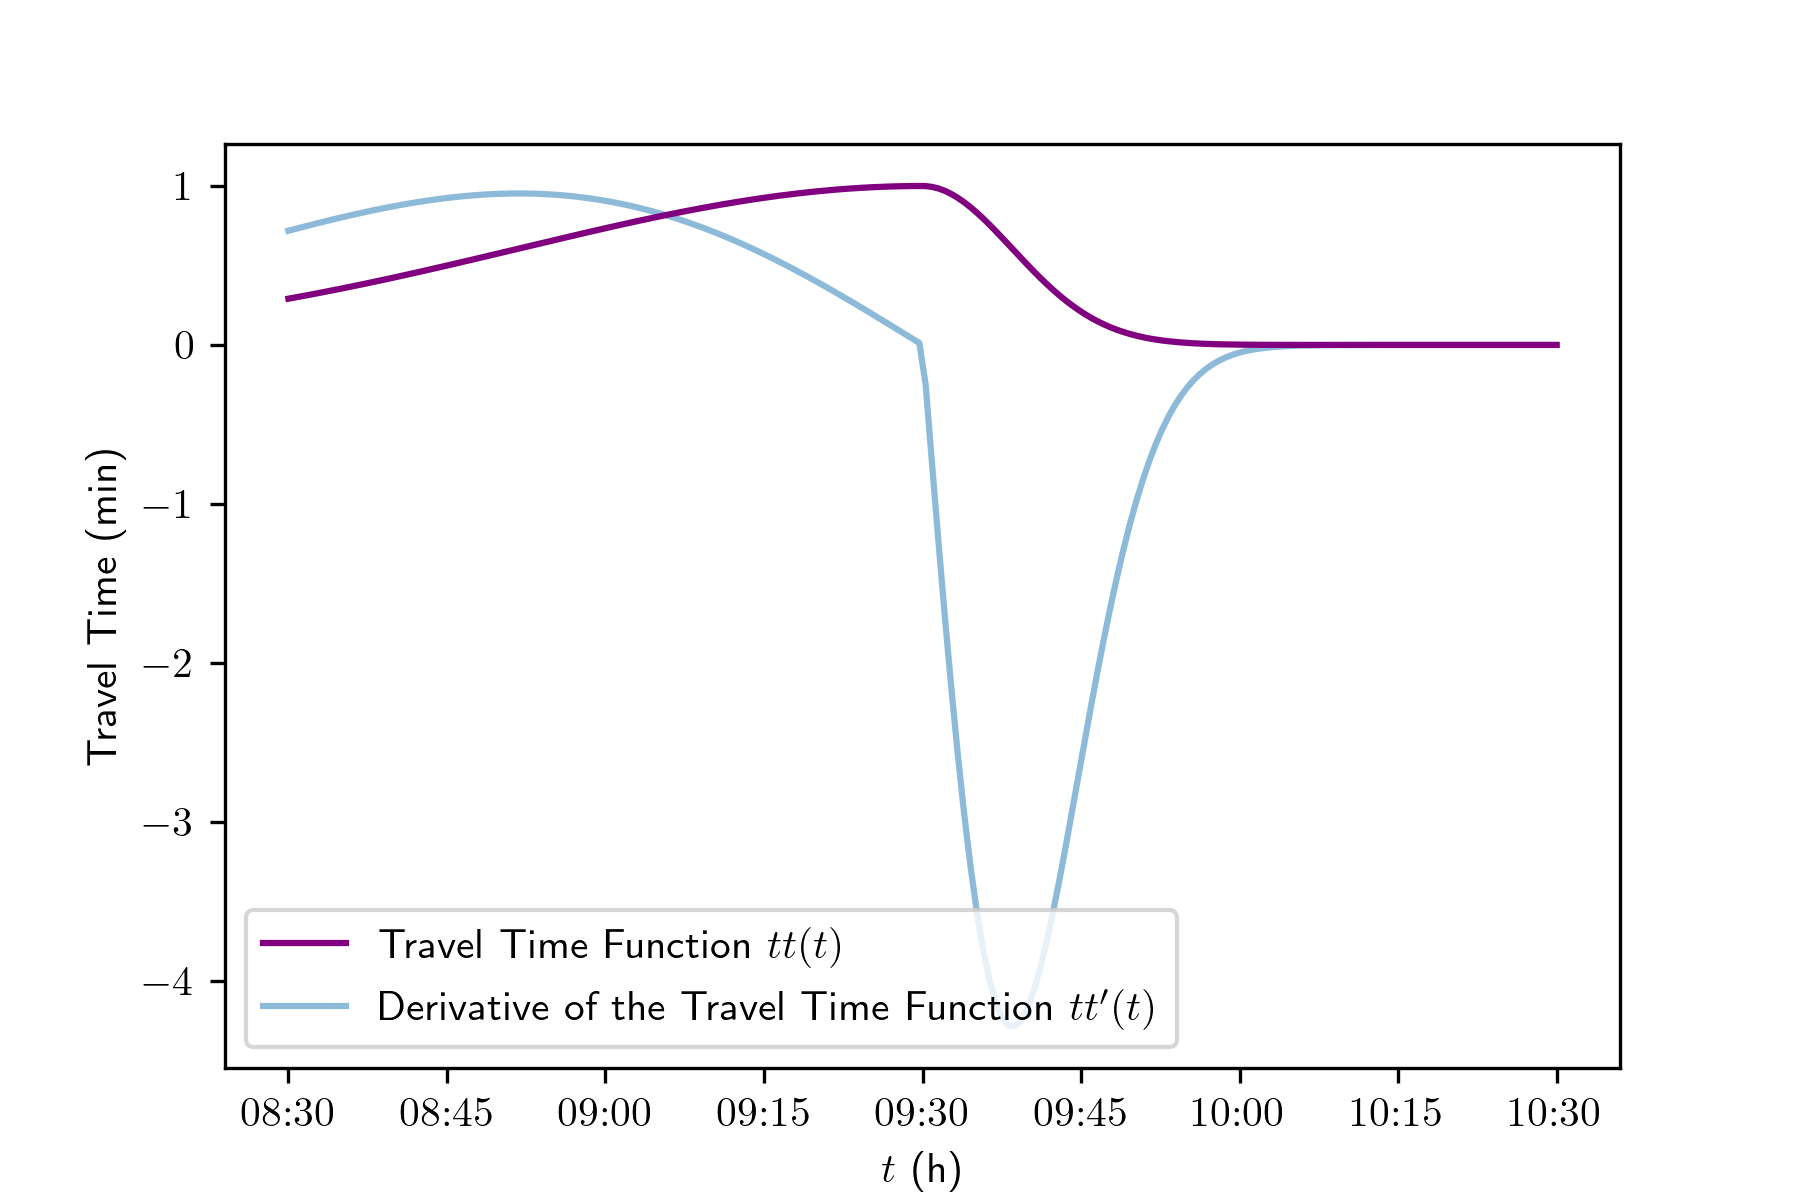
\includegraphics[width=.8\textwidth]{theo_tt}
  \caption{
    Example of a proper travel time function \(tt_a(t)\),
  plotted with its derivative.}
  \label{fig:theo_tt}
\end{figure}

But for a proper travel time function,
a point satisfying the conditions above can occur only once.
Given the unimodality,
the function will indeed be as shown in Figure~\ref{fig:theo_tt}: increasing, with an increasing derivative,
for \(t < k_1\), and decreasing with an increasing derivative for \(t > k_2\).
Its derivative will thus be injective on the convex part \(\mathcal{D}_{conv}\),
that is the only part in which the second derivative is non-negative.

Being the derivative injective,
there is at most one point \(t_i^e\) satisfying the condition \(tt_a(t_i^e) = \beta\).
The set \(E\) is thus either empty or a singleton.
A similar reasoning holds for late arrivals.

Consider thus now the problem of finding values for the bounds of the intervals \((t_i^e, t_f^e)\), \((t_i^l, t_f^l)\).
The points in which the arrivals occur are easy to estimate.

Let
\begin{align*}
  \beta_{max} = \max_t tt_a'(t) && \gamma_{max} = -\min_t tt_a'(t)
\end{align*}

The following functions are well defined:
\begin{equation}
  \label{eq:def-inv-der}
  \begin{aligned}
    t_i^e: (0, \beta_{max}) & \rightarrow \mathcal{D}_{conv}  & t_e^l: (0, \gamma_{max}) & \rightarrow \mathcal{D}_{conv} \\
    \beta & \mapsto (tt_a' |_{\mathcal{D}_{conv}})^{-1}(\beta) & \gamma & \mapsto(tt_a' |_{\mathcal{D}_{conv}})^{-1}(\gamma)
  \end{aligned}
\end{equation}
\begin{figure}
  \centering
  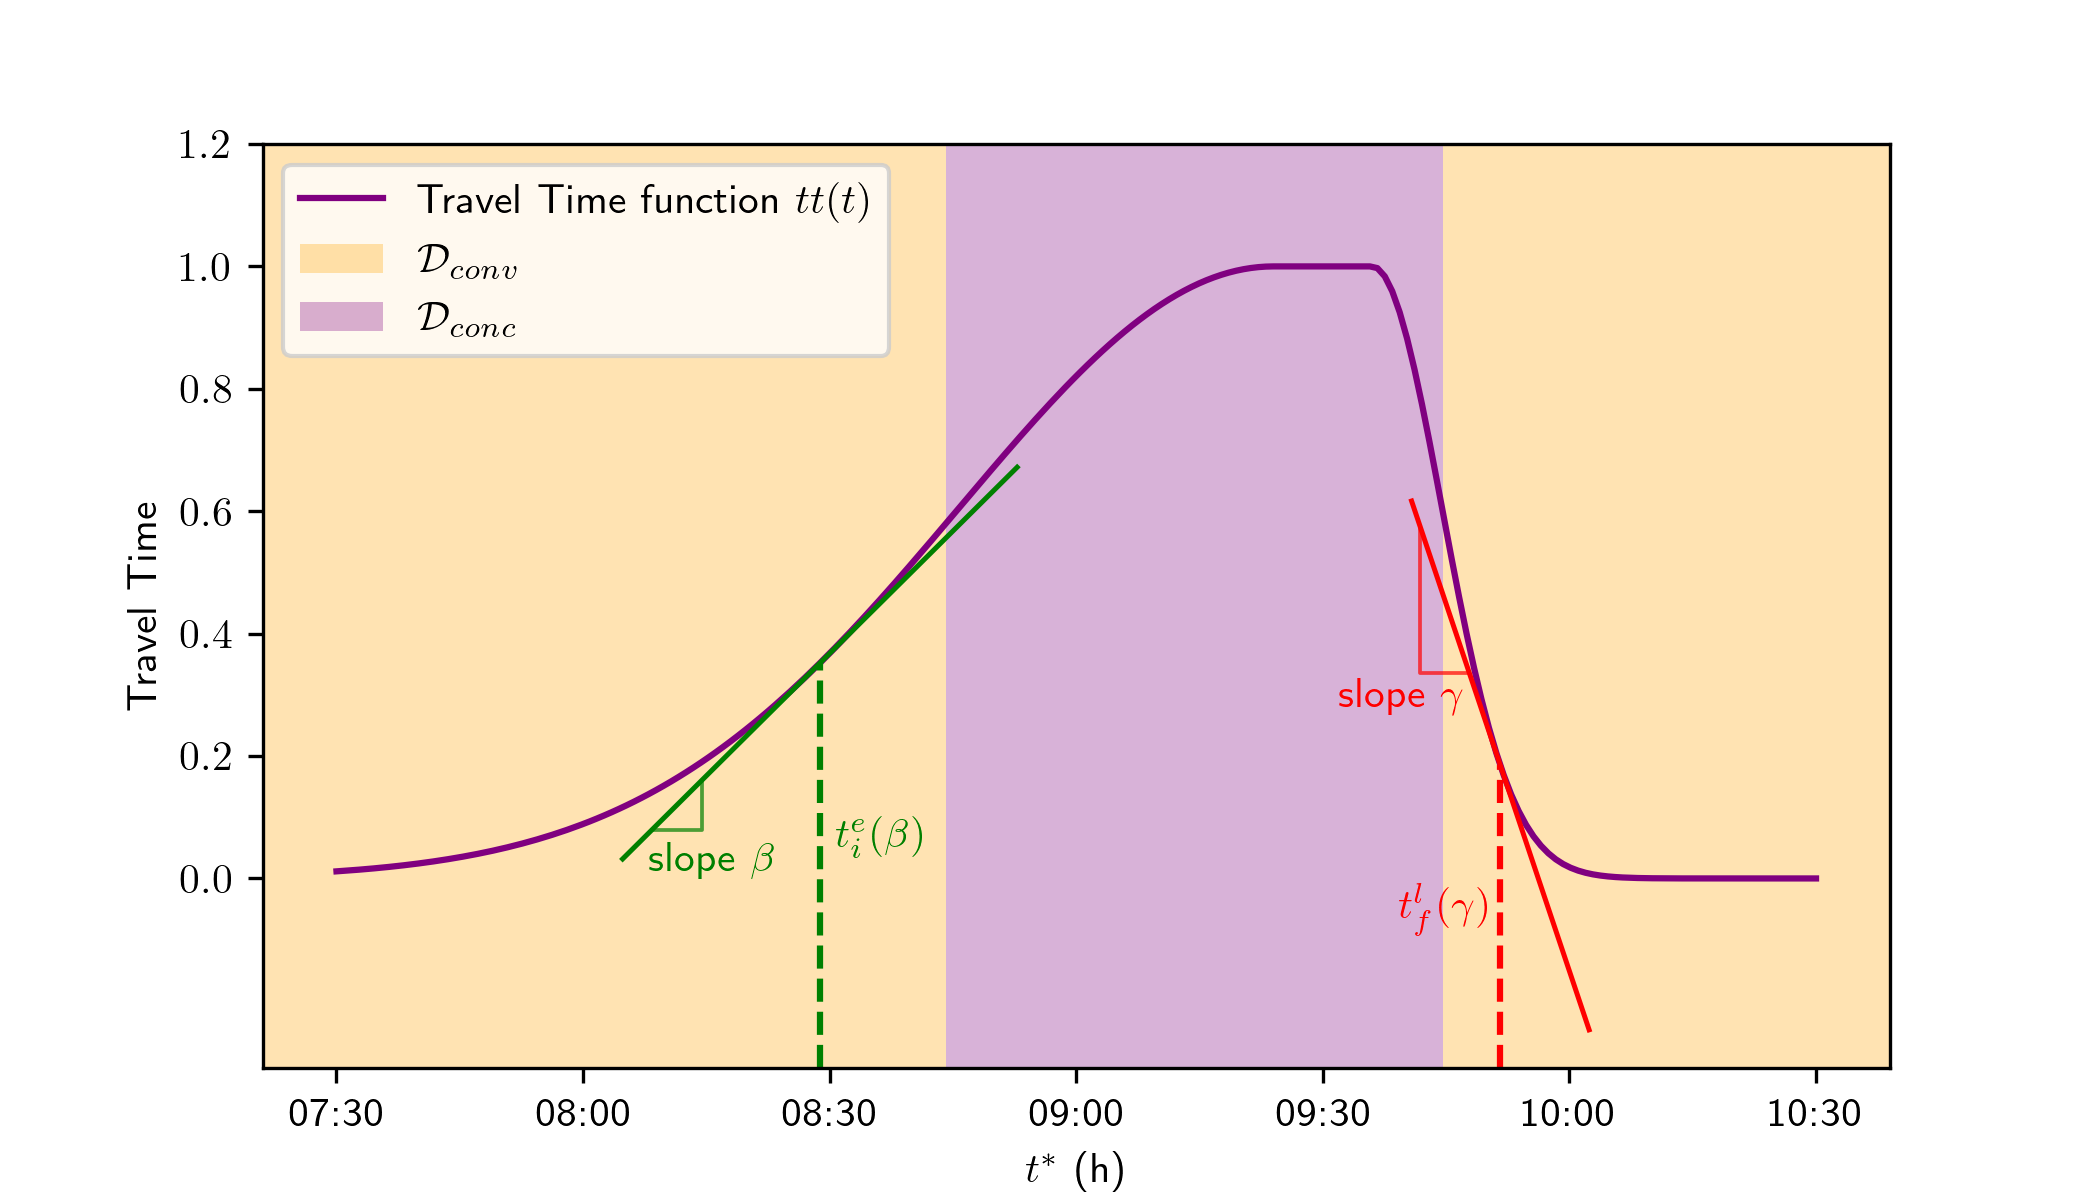
\includegraphics[width=.9\textwidth]{tang_cond}
  \caption{
    Proper travel time function,
    in which the results of the functions \(t_i^e(\beta), t_f^l(\gamma)\) are shown.
    The highlighted zones show the domains \(\mathcal{D}_{conc}, \mathcal{D}_{conv}\),
    that restrict the zones in which the derivative is inverted.
}
  \label{fig:tang-cond}
\end{figure}

Figure~\ref{fig:tang-cond} shows the outcomes of these functions on a theoretical proper travel time function

The functions \(t_i^e, t_f^l\) compute thus the initial point of the interval that yields early arrivals,
as well as the final point of the interval that yields late arrivals.

Estimating the remaining points \(t_f^e, t_i^l\) is slightly more difficult.
The expression in the proof of Proposition~\ref{prop:into-early-late} can anyway be used:
the function \(t_f^e(\beta), t_i^l(\gamma)\)
are thus defined as the points in which the line tangent to the travel time function at the initial points
(that are, the solid lines in Figure~\ref{fig:tang-cond})
intersect a second time with the travel time function.

\begin{figure}
  \centering
  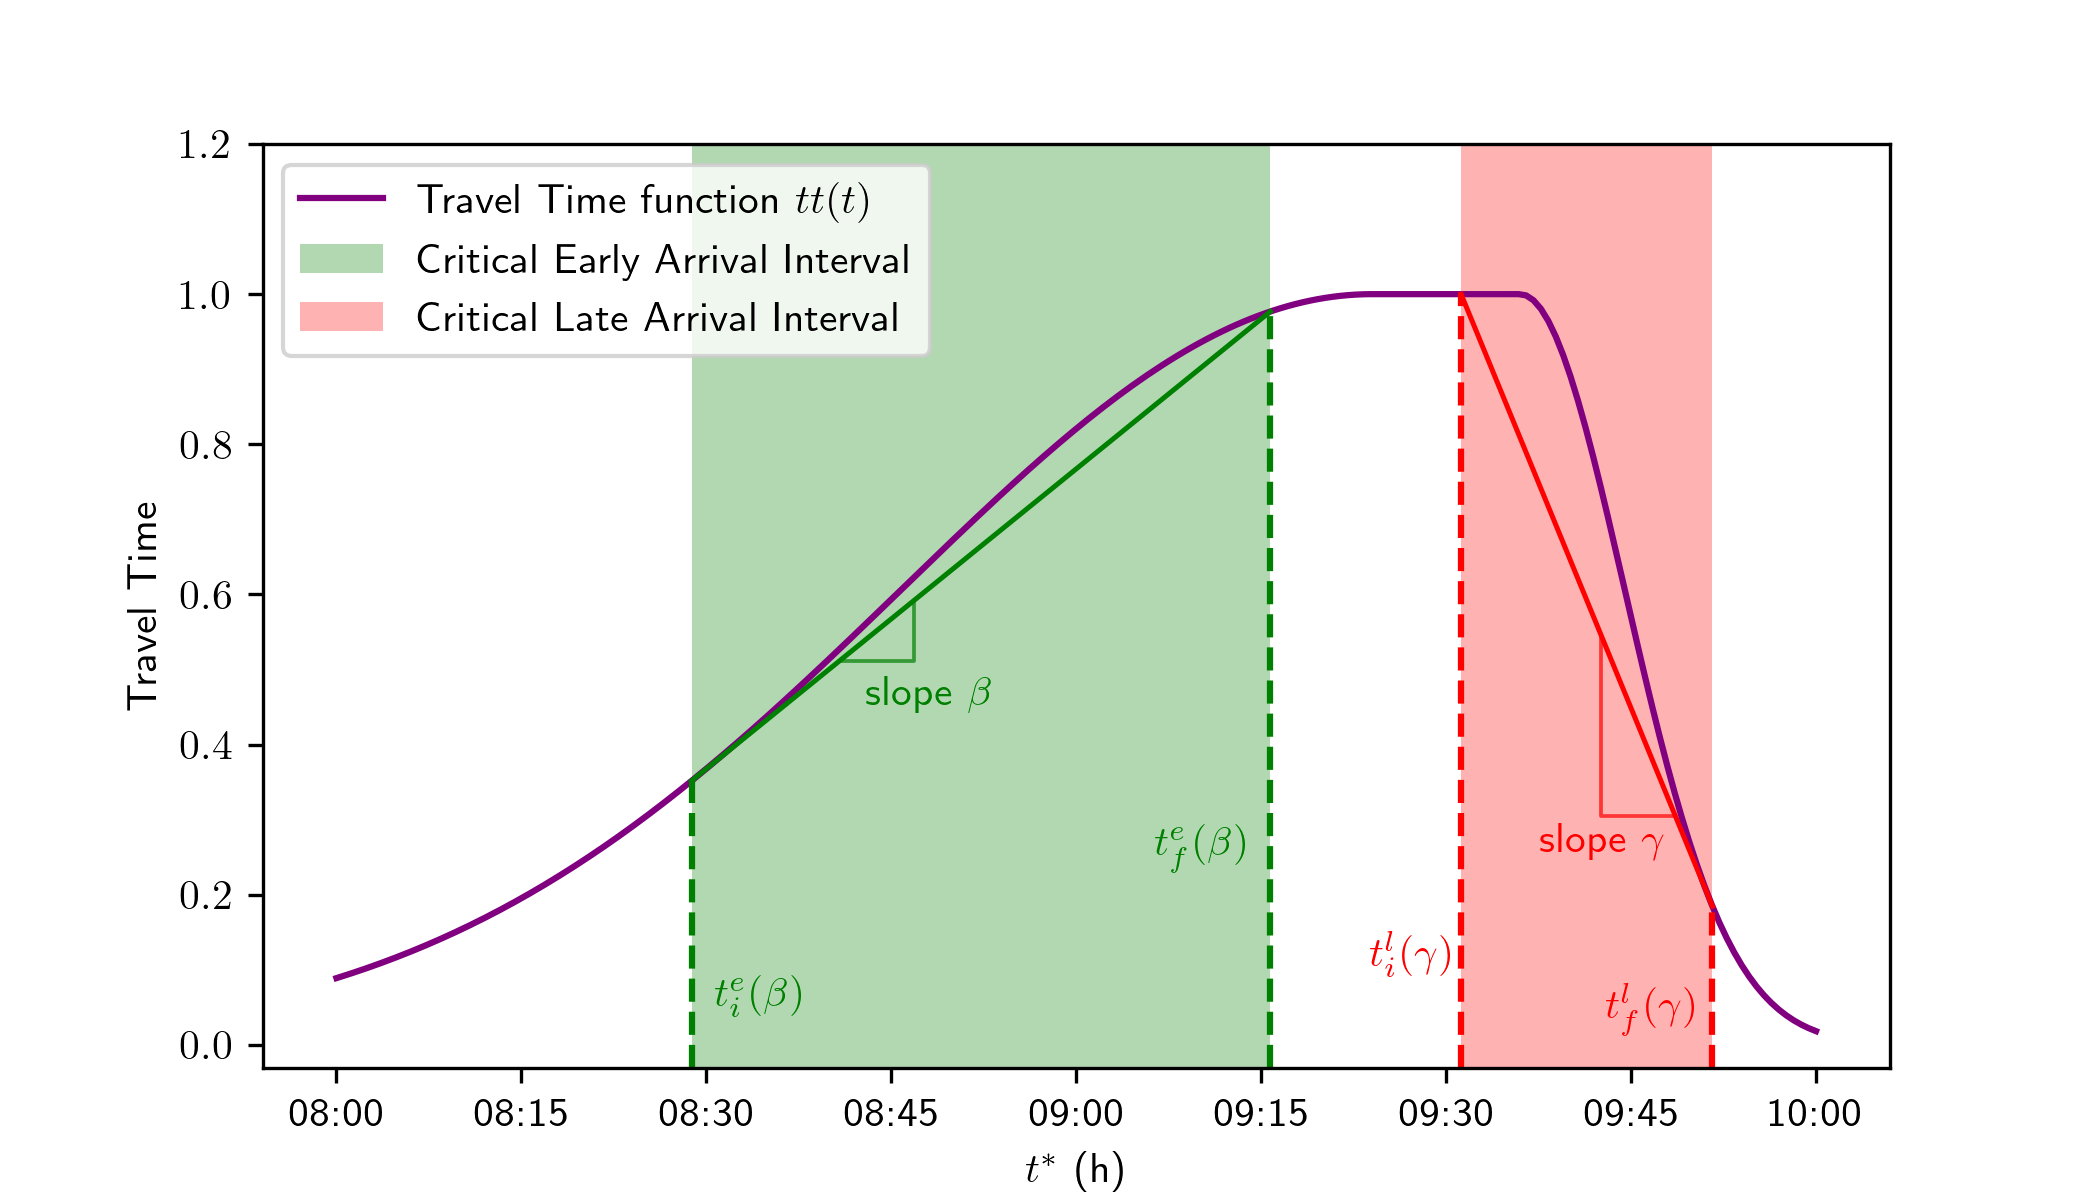
\includegraphics[width=.8\textwidth]{early_late_int}
  \caption{Outcomes of the functions \(t_i^e, t_f^e, t_i^l, t_f^l\),
    which define the bounds of the critical early and late intervals.
    The shaded zones show the so defined intervals,
  that yield an early or late arrival.}
  \label{fig:early-late-int}
\end{figure}

A graphical representation of the functions \(t_i^e, t_f^e, t_i^l, t_f^l\) is shown in Figure~\ref{fig:early-late-int}.
Once these functions have been defined,
the probability density function that characterizes the distribution of the optimal departure time \(t^{opt}\) can be computed.

\subsection{The Probability Density Function}

For considering the stochasticity in the cost minimization,
we will consider the parameters of the cost function to be random variables instead of deterministic parameters.
We thus consider the problem in which,
instead of the parameters \(\beta, \gamma, t^*\),
we consider three random variables \(B, \Gamma, T^*\).

A random variable for the optimal arrival will be defined as follows:
\begin{equation}
  \label{eq:rv-opt-arr}
  T^{opt} = t^{opt}(B, \Gamma, T^*)
\end{equation}

The goal of this section will be finding the probability density function \(f_{T^{opt}}\) of the variable \(T^{opt}\).

In order to simplify the estimation process, an assumption (which is, indeed, quite restrictive)
is made on these random variable:

\begin{assumption}
  The random variables \(B, \Gamma, T^*\) are pairwise independent
\end{assumption}

Note that this assumption is rather significant,
but not as significant as it may sound:
remind indeed that, being the parameter \(\alpha\) in equation~\eqref{eq:cost_ta} normalized to 1,
the parameters \(\beta, \gamma\) represent the values of the early and late arrival penalties normalized on the value of time,
rather than the raw parameters.
The assumption of independence is thus more realistic than how it was if the parameters were not normalized\todo{I need some help in better writing this}.

In the first place,
 it is convenient to distinguish between early, late and on-time arrivals.
In order to make this distinction, we define another random variable:
\begin{definition}
  Consider the function
  \begin{equation*}
    q(\beta, \gamma, t^*) =
    \begin{cases}
      -1 & \text{if } t^{opt}(\beta, \gamma, t^*) = t_e^{opt}(\beta, \gamma, t^*) \\
      0 & \text{if } t^{opt}(\beta, \gamma, t^*) = t^* \\
      1 & \text{if } t^{opt}(\beta, \gamma, t^*) = t_l^{opt}(\beta, \gamma, t^*)
    \end{cases}
  \end{equation*}

  Given the random variables \(B, \Gamma, T^*\), the random variable \(Q\) is defined as follows:
  \begin{equation*}
    Q  = q(B, \Gamma, T^*)
  \end{equation*}
\end{definition}

In practical terms, the random variable \(Q\) shows whether an early, on-time or late arrival is realized,
and takes the value \(-1\) if the optimal arrival is an early arrival,
\(1\) if it is a late arrival and \(0\) if it is an on-time one.

Since an optimal arrival can only be early, on-time or late,
by using the sum rule,
the probability density function for the random variable \(T^{opt}\) can be decomposed into three different parts:
\begin{equation}
  \label{eq:pdf-decomposed-q}
  f_{T^{opt}}(t) = f_{T^{opt}, Q}(t, -1) + f_{T^{opt}, Q}(t, 0) + f_{T^{opt}, Q}(t, 1)
\end{equation}
where \(f_{T^{opt}, Q}\) is the joint p.d.f for the random variables \(T^{opt}, Q\).

The single addends in~\eqref{eq:pdf-decomposed-q}
correspond to the density of early, on-time and late arrivals.
They are easier to individually describe,
and will be individually studied in the following.

\subsubsection{On-time Arrivals}

The value of the function
\begin{equation*}
  f_{T^{opt}, Q}(t, 0)
\end{equation*}
will be here computed.

Given a value for the arrival time \(t\),
the value of the function \(f_{T^{opt}, Q}(t, 0)\) represents how likely is the time \(t\) to be the outcome of an on-time arrival.

Note that Observation~\ref{obs:simplified-char} fully characterizes the values of the parameters for which the on-time arrivals are realized:
we are able, by using this characterization, to better describe the event at issue.

In particular, we note that the arrival time \(t\) is an optimal on-time arrival if and only if two conditions are satisfied at the same time:
the time \(t\) has to be a realization of the desired arrival time \(T^*\),
and it has to  be out from the intervals
\footnote{
  Note that \(E(B), L(\Gamma)\) are here sets of intervals rather than intervals.
  They can be, in this section, treated as intervals:
  Observation~\ref{obs:simplified-char} shows indeed that they can't contain more than a single interval.
}
\(E(B), L(\Gamma)\).

Being the random variable \(T^*\) independent from \(B, \Gamma\),
the two events above are independent and their likelihood can be multiplied:
\begin{equation}
  \label{eq:on-time-intro}
  f_{T^{opt}, Q}(t, 0) = f_{T^*}(t) \cdot \prob(t \notin E(B) \cup L(\Gamma))
\end{equation}
where \(f_{T^*}\) is the probability density function of the random variable \(T^*\), and is known.

Expression~\eqref{eq:on-time-intro} leads to a straightforward way of computing the desired value:
the probability of being out from the intervals \(E(B), L(\Gamma)\) can indeed be simply evaluated by integration:

\begin{equation}
  \label{eq:prob-not-intervals}
  \prob( t \not\in E(B) \cup L(\Gamma)) = \int_{b\in \R \vert t \not\in E(b)}\int_{g \in \R \vert t \not\in L(g)}f_B(b)f_\Gamma(g)\, dg\, db
\end{equation}
where \(f_B, f_\Gamma\) are the probability densities of, respectively, the random variables \(B, \Gamma\).


It is now possible to take advantage of Proposition\todo{Need to add this proposition somewhere...}:
the monotonicity of the intervals imply that there exist two functions representing the maximum values that \(\beta\) and \(\gamma\) can assume while keeping a given point into the defined intervals:
\begin{equation}
  \label{eq:def_b_0_g_0}
  \begin{split}
    \beta_0:\R&\rightarrow(0, \beta_{max}] \\
    t&\mapsto \sup\{b | t \in E(b)\} \\[1em]
    \gamma_0:\R&\rightarrow(0, \gamma_{max}] \\
    t&\mapsto \sup\{g | t \in L(g)\}
  \end{split}
\end{equation}

The definition of these functions simplifies the integrals in~\eqref{eq:prob-not-intervals}, that become

\begin{equation}
  \label{eq:on-time-monot}
  \prob( t \not\in E(B) \cup L(\Gamma)) = \int_{\beta_0(t)}^{\beta_{\text{max}}}\int_{\gamma_0(t)}^{\gamma_{\text{max}}}f_B(b)f_\Gamma(g)\, dg\, db
\end{equation}

By exploiting the expression obtained in equation~\eqref{eq:on-time-monot},
the joint probability density functions in equation~\eqref{eq:on-time-intro} can be analytically evaluated:
\begin{equation}
  \label{eq:on-time-final}
  \begin{split}
    f_{T^{opt}, Q}(t, 0) & = f_{T^*}(t) \cdot \prob(t \notin E(B) \cup L(\Gamma)) \\
    & = f_{T^*}(t)\int_{\beta_0(t)}^{\beta_{\text{max}}}\int_{\gamma_0(t)}^{\gamma_{\text{max}}}f_B(b)f_\Gamma(g)\, dg\, db
  \end{split}
\end{equation}

Note that all the functions used in the right hand side can be evaluated.
This concludes thus the evaluation of the likelihood of being an on-time arrival.
In the following part, the likelihood of being an early or late arrival will be described.

\subsubsection{Early and Late Arrivals}

Before discussing the case of early and late arrivals,
the following definition,
which gives a simpler way to separate the early arrivals from the late arrivals,
is given:

\begin{definition}
  \label{def:intervals-tilde}
  We denote as \(\tilde{E}(\beta, \gamma), \tilde{L}(\beta, \gamma)\) the intervals which yield early or late arrivals:
  \begin{align*}
    \tilde{E}(\beta, \gamma) & = (t_i^e(\beta), \min\{t_f^e(\beta), t_s(\beta, \gamma)\})\\
    \tilde{L}(\beta, \gamma) & = (\max\{t_i^l(\gamma), t_s(\beta, \gamma)\}, t_f^l(\gamma))
  \end{align*}
\end{definition}

Note that the intervals are necessarily disjoint,
since the ending point of the interval \(\tilde{E}\) is lower or equal to the starting point of \(\tilde{L}\).

Moreover,
the optimal arrival time \(t^{opt}(\beta, \gamma, t^*)\) will be an early (or late) arrival
if and only if the desired arrival time \(t^*\)
is in the interval \(\tilde{E}(\beta, \gamma)\) (respectively, \(\tilde{L}(\beta, \gamma)\)).

Another assumption is now made on the distributions of the variables \(B, \Gamma\):

\begin{assumption}
  \label{ass:domain-rv}
  The random variables \(B, \Gamma\) are entirely supported, respectively,
  into the intervals \((0, \beta_{max})\), \((0, \gamma_{max})\),
  that is
  \begin{align*}
    \int_0^{\beta_{max}}f_B(b) db = 1 && \int_0^{\gamma_{max}}f_\Gamma(g) dg = 1
  \end{align*}
\end{assumption}

Note that this assumption is quite restrictive,
and contrasts with recent literature \cite[see][]{hall2024inframarginal}.
It is anyway useful while developing the theory,
and will be dropped in a later stage.

Consider thus now the value of the function
\begin{equation*}
  f_{T^{opt}, Q}(t, -1)
\end{equation*}

Observation NUMBER shows that the arrival time \(t\) is an early arrival if and only if two conditions,
similar to the ones in the preceding case,
are realized:
the time \(t\) has to be a realization of the optimal early arrival time \(t_i^e(B)\) and,
on top of this, it has to be into the interval \(\tilde{E}(B, \Gamma)\).

Differently from the case about on-time arrivals,
the random variable \(B\) appears in both conditions:
the events are thus not independent anymore,
and their joint density will be computed via its decomposition in conditional densities:
\begin{equation}
  \label{eq:late-joint-decomp}
  f_{T^{opt}, Q}(t, -1) = \prob\left(T^* \in \tilde{E}(B, \Gamma)|\, t_i^e(B) = t\right) f_{t_i^e(B)}(t)
\end{equation}
where \(f_{t_i^e(B)}(t)\) is the probability density function for the random variable \(t_i^e(B)\).
The density is computed in the following lemma:
\begin{lemma}
  \label{lemma:transformed-B}
  Let \(t_i^e\) be the function defined in~\eqref{eq:def-inv-der}, \(B\) a random variable with probability density function \(f_B\),
  satisfying Assumption~\ref{ass:domain-rv}.
  
  The probability density function \(f_{t_i^e(B)}\) for the transformed random variable \(t_i^e(B)\) is given by
  \begin{equation*}
    f_{t_i^e(B)}(t) = f_B(tt_a'(t)) [tt_a''(t)]^+
  \end{equation*}
  where
  \begin{equation*}
    [x]^+ = \max\{x, 0\}
  \end{equation*}
\end{lemma}

\begin{proof}
  Note at first that the function
  \begin{equation*}
    \beta \mapsto t_i^e(\beta)
  \end{equation*}
  coincides, on its domain,
with the inverse of the travel time function derivative, and is thus a bijection.
In \citet{casella2001statistical}, Theorem 2.1.5 shows how to compute in this case the p.d.f. of the transformed random variable \(t_i^e(B)\):
\begin{equation}
  \label{eq:pdf-b-change-var}
  f_{t_i^e(B)}(t) =
  \begin{cases}
    f_B((t_i^e)^{-1}(t)) \left| \diff{}{t}((t_i^e)^{-1}(t)) \right| & \text{if } t \in t_i^e\left(\text{supp}(f_B)\right) \\
    0 & \text{otherwise}
  \end{cases}
\end{equation}
where \(\text{supp}(f_B)\) is the support of the probability density function \(f_B\), that is
\begin{equation*}
  \text{supp}(f_B) = \{b \in \R |\, f_B(b) > 0 \}
\end{equation*}

Note now that Assumption~\ref{ass:domain-rv} holds:
\(\text{supp}(f_B)\) is thus in the domain of the function \(t_i^e\),
and equation~\eqref{eq:pdf-b-change-var} is well defined.

Since times that are out of the image of the function \(t_i^e\) are,
not considered,
we can set
\begin{equation*}
  (t_i^e)^{-1}(t) = tt_a'(t)
\end{equation*}

Moreover, being the function \(t_i^e\) invertible on its whole domain,
the two cases in equation~\eqref{eq:pdf-b-change-var} are equally well defined and coincide for \(t = t_i^e(b), f_B(b) = 0\).
The density function for the transformed random variable will thus be
\begin{equation*}
  f_{t_i^e(B)}(t) =
  \begin{cases}
    f_B(tt_a'(t)) \left|tt_a''(t)\right| & \text{if } t \in t_i^e\left((0, \beta_{max})\right) \\
    0 & \text{otherwise}
  \end{cases}
\end{equation*}

Note now that the second case is necessary only if the travel time function is concave,
since assumption~\ref{ass:domain-rv} ensures that the two expression coincide for \(tt_a'(t) \leq 0\).

The syntax can thus be simplified by writing
\begin{equation*}
  f_{t_i^e(B)}(t) = f_B(tt_a'(t)) [tt_a''(t)]^+
\end{equation*}
where the employment of the function \([\bullet]^+\) ensures that,
when the travel time function is concave (that is, its second derivative \(tt_a''(t)\) is negative),
the density is equal to zero.
\end{proof}

An explicit expression for the density \(f_{t_i^e(B)}\) has thus been found.
In the following, we will study the probability
\begin{equation*}
  \prob\left(T^* \in E(B, \Gamma)|\, t_i^e(B) = t\right)
\end{equation*}

The condition \(t_i^e(B) = t\) implies, by definition of \(t_i^e\),
\begin{align*}
  B & = (t_i^e)^{-1}(t) \\
    & = tt_a'(t)
\end{align*}

By substituting these in the original expression, we get
\begin{equation}
  \label{eq:early-subst}
  \begin{split}
    f_{T^{opt}, Q}(t, -1) & = \prob(T^* \in E(tt_a'(t), \Gamma))f_{t_i^e(B)}\\
    & = \prob(T^* \in (t, \min\{t_f^e(tt_a'(t)), t_s(tt_a'(t), \Gamma)\}))f_{t_i^e(B)}(t)
  \end{split}
\end{equation}

Integrating the random variables,
and substituting what found in Lemma~\ref{lemma:transformed-B},
yields an explicit expression for the desired probability density function:
\begin{equation}
  \label{eq:early-final}
  f_{T^{opt}, Q}(t, -1) = \int_0^\infty \int_t^{\min\{t_f^e(tt_a'(t)), t_s(tt_a'(t), g)\}}f_{T^*}(s) f_\Gamma(g)\ ds\ dg f_B(tt_a'(t)) [tt_a''(t)]^+
\end{equation}

For the late arrivals, an analogous reasoning finds a similar expression:
\begin{equation}
  \label{eq:late-final}
  f_{T^{opt}, Q}(t, 1) = \int_0^\infty \int_t^{\max\{t_i^l(-tt_a'(t)), t_s(b, -tt_a'(t))\}}f_{T^*}(s) f_B(b)\ ds\ db f_B(tt_a'(t)) [tt_a''(t)]^+
\end{equation}

This last expression terminates the possible values for the variable \(Q\),
and allows us to write an expression for the probability density function of the variable \(T^{opt}\) alone.

\subsubsection{Expression for the Probability Density Function}

By substituting the expressions found for the joint probabilities in equation~\eqref{eq:pdf-decomposed-q},
we find the following:
\begin{multline}
  \label{eq:pdf-final}
    f_{T^{opt}}(t) = f_{T^*}(t)\int_{\beta_0(t)}^{\beta_{\text{max}}}\int_{\gamma_0(t)}^{\gamma_{\text{max}}}f_B(b)f_\Gamma(g)\, dg\, db \\
    + \int_0^\infty \int_t^{\min\{t_f^e(tt_a'(t)), t_s(tt_a'(t), g)\}}f_{T^*}(s) f_\Gamma(g)\ ds\ dg f_B(tt_a'(t)) [tt_a''(t)]^+ \\
    + \int_0^\infty \int_t^{\max\{t_i^l(-tt_a'(t)), t_s(b, -tt_a'(t))\}}f_{T^*}(s) f_B(b)\ ds\ db f_B(tt_a'(t)) [tt_a''(t)]^+
\end{multline}

Given the probability density functions according to which the scheduling preferences parameters \(\beta, \gamma\) and the desired arrival time \(t^*\) are distributed,
this expression allows thus the direct computation of the distribution of the optimal arrival time \(t^{opt}\),
which minimizes the cost faced by the traveller when choosing a departure time.

If we suppose the distributions of the parameters to be parametrized by some parameter \(\theta\),
this allows a Maximum Likelihood Estimation of the parameter,
that will be performed in the following.

\subsection{MLE Configuration}

The expression found in equation~\eqref{eq:pdf-final} can be used to perform a Maximum Likelihood Estimation,
to estimate a parameter that has an impact on the distribution of the random variables \(B, \Gamma, T^*\).

Suppose thus the distribution of the random variables being dependant on a parameter \(\theta \in \R^d\):
\begin{align*}
  B \sim f_B(x; \theta) && \Gamma \sim f_\Gamma(x; \theta) && T^* \sim f_{T^*}(t; \theta)
\end{align*}

The probability density function in equation~\eqref{eq:pdf-final} will itself depend on the parameter \(\theta\):
\begin{equation*}
  f_{T^{opt}}(t) = f_{T^{opt}}(t; \theta)
\end{equation*}

By fixing the parameter \(\theta\),
the likelihood of an observed arrival time \(t_0\) can be computed:
\begin{equation}
  \label{eq:lik-single}
  \mathcal{L}(\theta | t) = f_{T^{opt}}(t; \theta)
\end{equation}

If a dataset of observations is given
\begin{equation*}
  T = \{t_i\}_i
\end{equation*}
the definition of the likelihood given in~\eqref{eq:lik-single} can be extended to the whole dataset:
\begin{equation}
  \label{eq:lik-final}
  \mathcal{L}(\theta | T) = \prod_i \mathcal{L}(\theta | t_i)
\end{equation}

An estimate \(\hat{\theta}\) for the parameter \(\theta\) will thus be found by maximising the likelihood:
\begin{equation}
  \label{eq:max-lik}
  \hat{\theta} = \argmax \mathcal{L}(\theta | T)
\end{equation}

%%% Local Variables:
%%% mode: LaTeX
%%% TeX-master: "../main"
%%% End:
